\documentclass[a4paper,10pt]{article}
\usepackage[utf8]{inputenc}
\usepackage[brazilian]{babel}
\usepackage{cite}
\bibliographystyle{plain}
\usepackage{hyperref}
\usepackage{indentfirst}
\usepackage{url}
\usepackage{graphicx}
\usepackage{wrapfig}
\usepackage{caption}
\usepackage{amsmath}
\usepackage{enumerate}
\usepackage{placeins}

%opening
\title{RELATÓRIO 1 - VARIÁVEIS ESPAÇOS-TEMPORAIS DA MARCHA}
\author{Camila Takano, Damiana A. Santos, João Oda}

\begin{document}

\maketitle

\begin{abstract}
Este relatório descreve o procedimento experimental e os resultados obtidos na primeira experiencia da disciplina Princípios e Aplicações de Biomecânica, Turma: EN2308
\end{abstract}

\section{Introdução}
As medidas espaço temporais da marcha podem ser adquiridas de forma simples possibilitando uma primeira analise do movimento e constituindo uma fonte importante de informação.

\section{Método}

\subsection{Participantes}
Neste experimentos foram obtidos dados de três indivíduos na faixa etária 20 a 30 anos, denominados doravante \textbf{C}, \textbf{D} e \textbf{J}. Sendo \textbf{C} e \textbf{D} do sexo feminino e \textbf{J} do sexo masculino. 

\subsection{Procedimento Experimental}
O comprimento do membro inferior dos participantes foi medido, sendo a distância do 
Maléolo Medial até Espinha Ilíaca Ântero-Superior.

Uma região de 15m de comprimento foi delimitada, por onde os participantes andam em trajetória aproximadamente retilínea a uma velocidade hipoteticamente constante, para atingir a velocidade constante um trecho de 5m é previamente percorrido. Ao tocar com o pé na região delimitada, inicia-se a cronometragem de tempo e a contagem de passos(a partir do $1^o$) ao pisar fora da região para-se se o cronômetro e a contagem de passos é encarrada. Cada um dos participantes é submetido a este procedimento três vezes, cada vez com uma ritmo/velocidade(Lento, Confortável e Rápido)

\section{Resultados}

\begin{table}
\label{tab_medidas}
\begin{center}
\begin{tabular}{l|ccc|ccc}
 & \multicolumn{3}{|c|}{N$^o$ de Passos} & \multicolumn{3}{|c}{Tempo(s)}\\
 velocidade & \textbf{C} & \textbf{D} & \textbf{J} & \textbf{C} & \textbf{D} & \textbf{J}\\
 \hline
Lenta & 26 & 26 & 24 & 14.06 & 13.66 & 17.37\\
Confortável & 24 & 24 & 18 & 10.94 & 12.44 & 12.66\\
Rápida & 18 & 20 & 14 & 7.91 & 8.97 & 6.82
\end{tabular}
\end{center}
\caption{Dados Medidos}
\end{table}



\begin{table}
\label{tab_calculados}
\begin{center}
\begin{tabular}{ll|lcccc}
&L(m)&velocidade & CD(passos/s) & CP(m) & Va(m/s) & Vb(m/s)\\
\hline
 & &Lenta & 1.85 & 0.58 & 1.07 & 1.07\\
\textbf{C}& 0,8&Confortável & 2.19 & 0.62 & 1.37 & 1.37\\
 & &Rápida & 2.28 & 0.83 & 1.90 & 1.90 \\
\hline
 & &Lenta & 1.90 & 0.58 & 1.10 & 1.10\\
\textbf{D}& 0,82&Confortável & 1.93 & 0.62 & 1.21 & 1.21\\
 & &Rápida & 2.23 & 0.75 & 1.67 & 1.67\\
\hline
 & &Lenta & 1.38 & 0.62 & 0.86 & 0.86\\
\textbf{J}& 1,0&Confortável & 1.42 & 0.83 & 1.18 & 1.18\\
 & &Rápida & 2.05 & 1.07 & 2.20 & 2.20\\
\end{tabular}
\end{center}
\caption{Váriaveis Calculadas}
\end{table}

\begin{figure}[h]
\label{plotCDxVa}
 \centering
 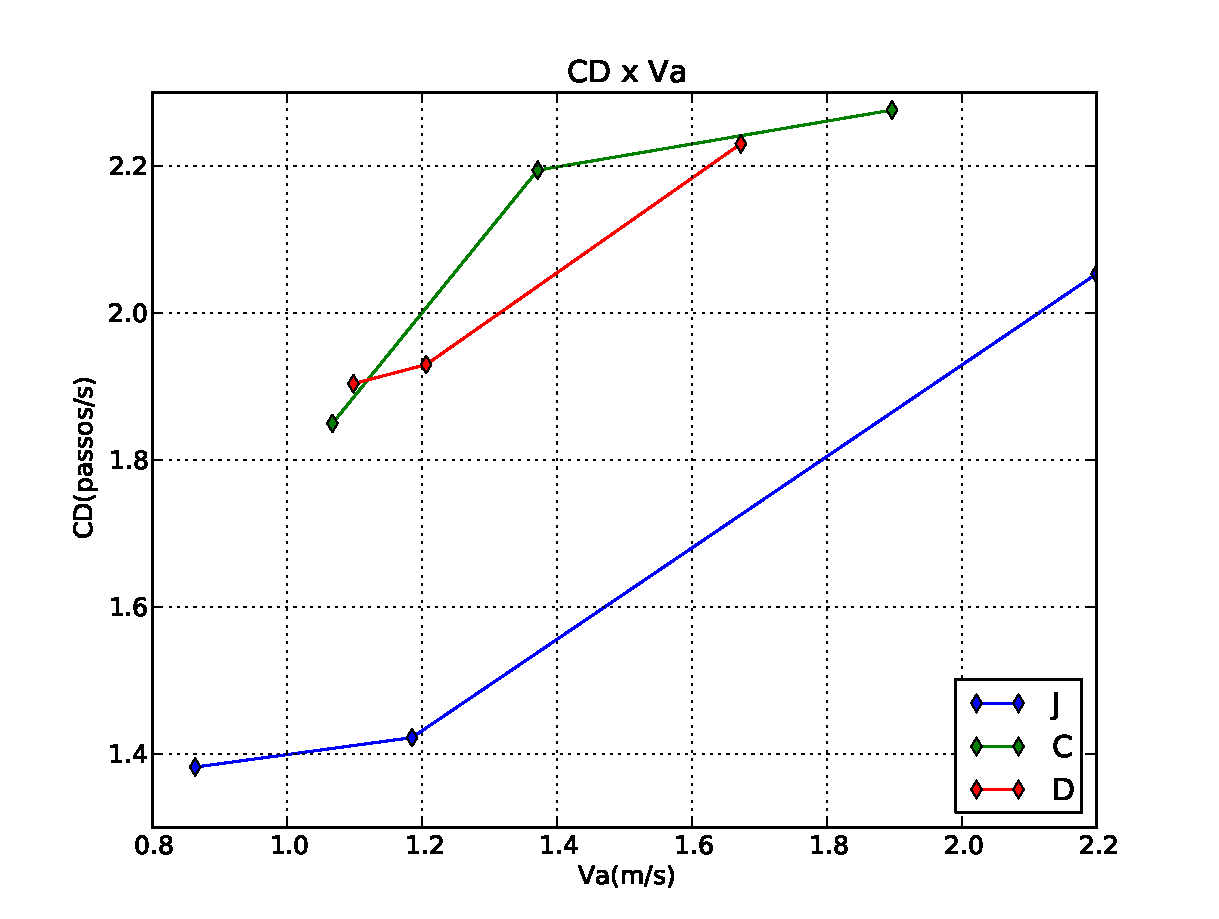
\includegraphics[scale=0.5,keepaspectratio=true]{./plot_CDxVa.pdf}
 % plot_CDxVa.pdf: 585x441 pixel, 72dpi, 20.64x15.56 cm, bb=0 0 585 441
 \caption{Gráfico Cadência de passos(CD) pela Velocidade do Andar(Va)}
\end{figure}

\begin{figure}[h]
\label{plotCPxVa}
 \centering
 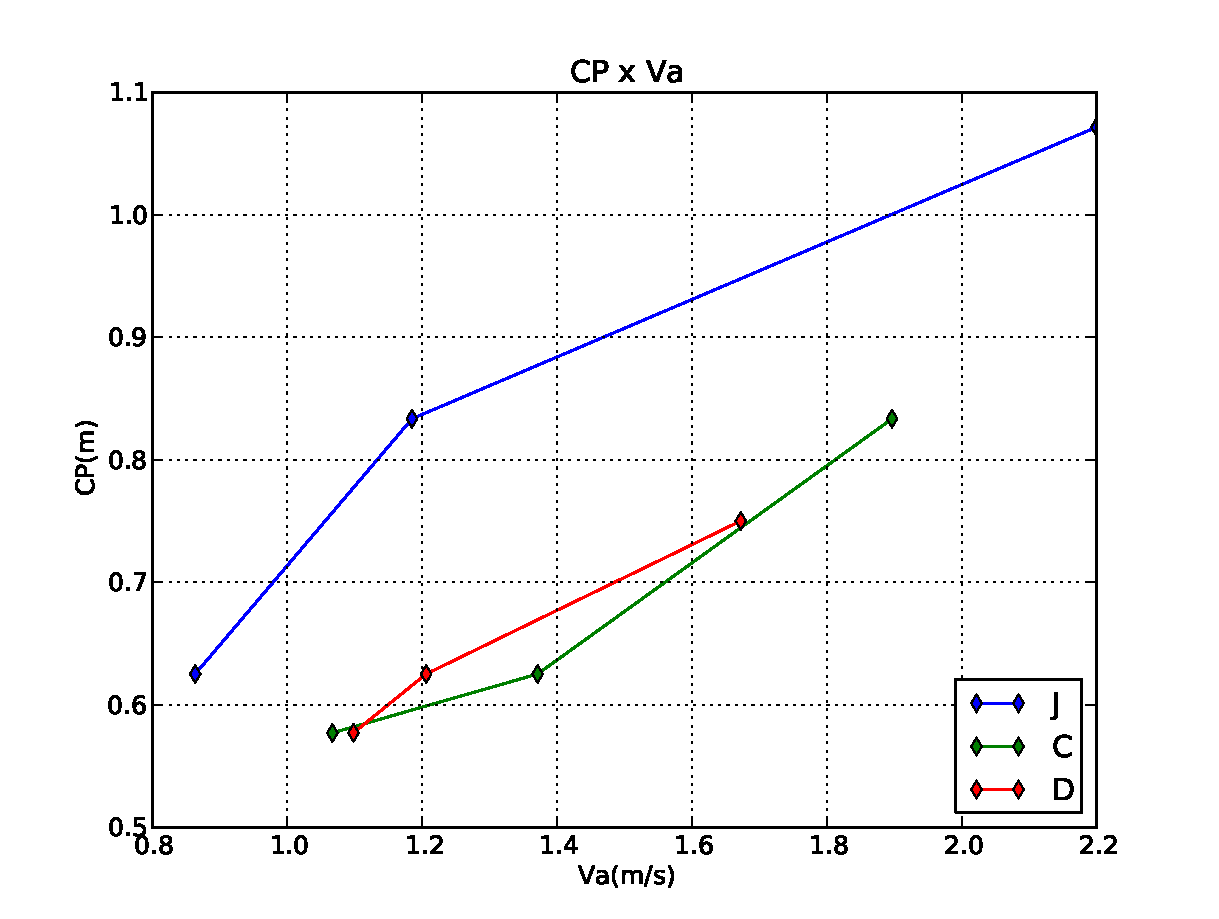
\includegraphics[scale=0.5,keepaspectratio=true]{./plot_CPxVa.pdf}
 % plot_CDxVa.pdf: 585x441 pixel, 72dpi, 20.64x15.56 cm, bb=0 0 585 441
 \caption{Gráfico Comprimento do passos(CP) pela Velocidade do Andar(Va)}
\end{figure}


\section{Discussão}



\end{document}
